\chapter{Prosessdokumentasjon}
%\marginpar{
%Test for sitering av kilder.\cite{forelesning:tulpesh}\cite{book:utforming}\cite{book:desintsystems}
%}
\lettrine[lines=2]{F}{} ølgende kapittel beskriver hvordan hele utviklingsprosessen av prototypene har foregått og som illustrerer hele prosessen fra idé til mockup til hi-hi prototype. Kapittelet består av mange bilder for å på enklest mulig måte illustrere prosessen. For eventuell beskrivelse av funksjonalitet av de modulene som er synlige på bildene henvises det til appendiks \ref{app:funksjonalitet}.




\section{Første utkast} \label{sec:utkast}
\marginpar{Viktige prinsipper:
feedback, constraints (bruker får ikke gjøre feil), affordances
}
\marginpar{Husk at vi borde ta med en navigasjonkart}
\marginpar{Støtteord:
Usability (brukbarhet): konsistens, brukerkontroll, passende presentasjon.
}
Etter at idéen om hva vi skulle jobbe med var klar tok det ikke lang tid før vi ble enige om hvordan vi skal sette sammen vårt forslag til en helhet. Hele gruppen var tydelig på at vi i stor grad ønsket å benytte oss av en løsning som følger Gestalt-prinsipper for god design og layout.
Systemet skulle kunne administreres via nettleser som gjør det mulig å bruke systemet fra hvilken som helst maskin og med eventuelle tilpasninger kan også gjøres slik at man også kan jobbe fra nettbrett eller telefon.
På det tidspunktet handlet diskusjonen om hvordan vi skulle fordele de forskjellige modulene og funksjonalitetene på så få hovedområder som mulig, der hvert av de områdene blir et element i hovedmenyen. 
I det første utkastet bestod disse av:
%\begin{center}
%\texttt{Editorer | Meldinger | Resurser | System | Servere}
%\end{center}
\begin{table}[h]
\newcommand{\paddA}{1ex}
\newcommand{\paddB}{0.2ex}
\begin{tabularx}{\textwidth}{|*5{>{\centering\arraybackslash}X|}@{}|}
\hline
\vspace*{\paddA} Editorer & \vspace*{\paddA} Meldinger & \vspace*{\paddA} Resurser & \vspace*{\paddA} System & \vspace*{\paddA} Servere \\[2ex] 
\hline
\vspace*{\paddB} Java		&	\vspace*{\paddB} HTML Val			& 	\vspace*{\paddB} Meldinger 	& 	\vspace*{\paddB} Apache 	& \vspace*{\paddB} Brannmur \\
PHP		& 	CSS Validering 	& 				& 	MySQL 	& Brukergrupper \\
MySQL	& 	W3Schools 		& 				& 	SSH 		& Logg \\
C 		& 	DropBox 			& 				& 			& Filbehnadling \\
 		& 	Terminal \vspace*{\paddB} 		& 				& 			& Systeminfo \vspace*{\paddB} \\

\hline
\end{tabularx} 
\end{table}


\begin{figure}
%bruk \begin{figure}[ht] dersom figuren ikke skal flyte
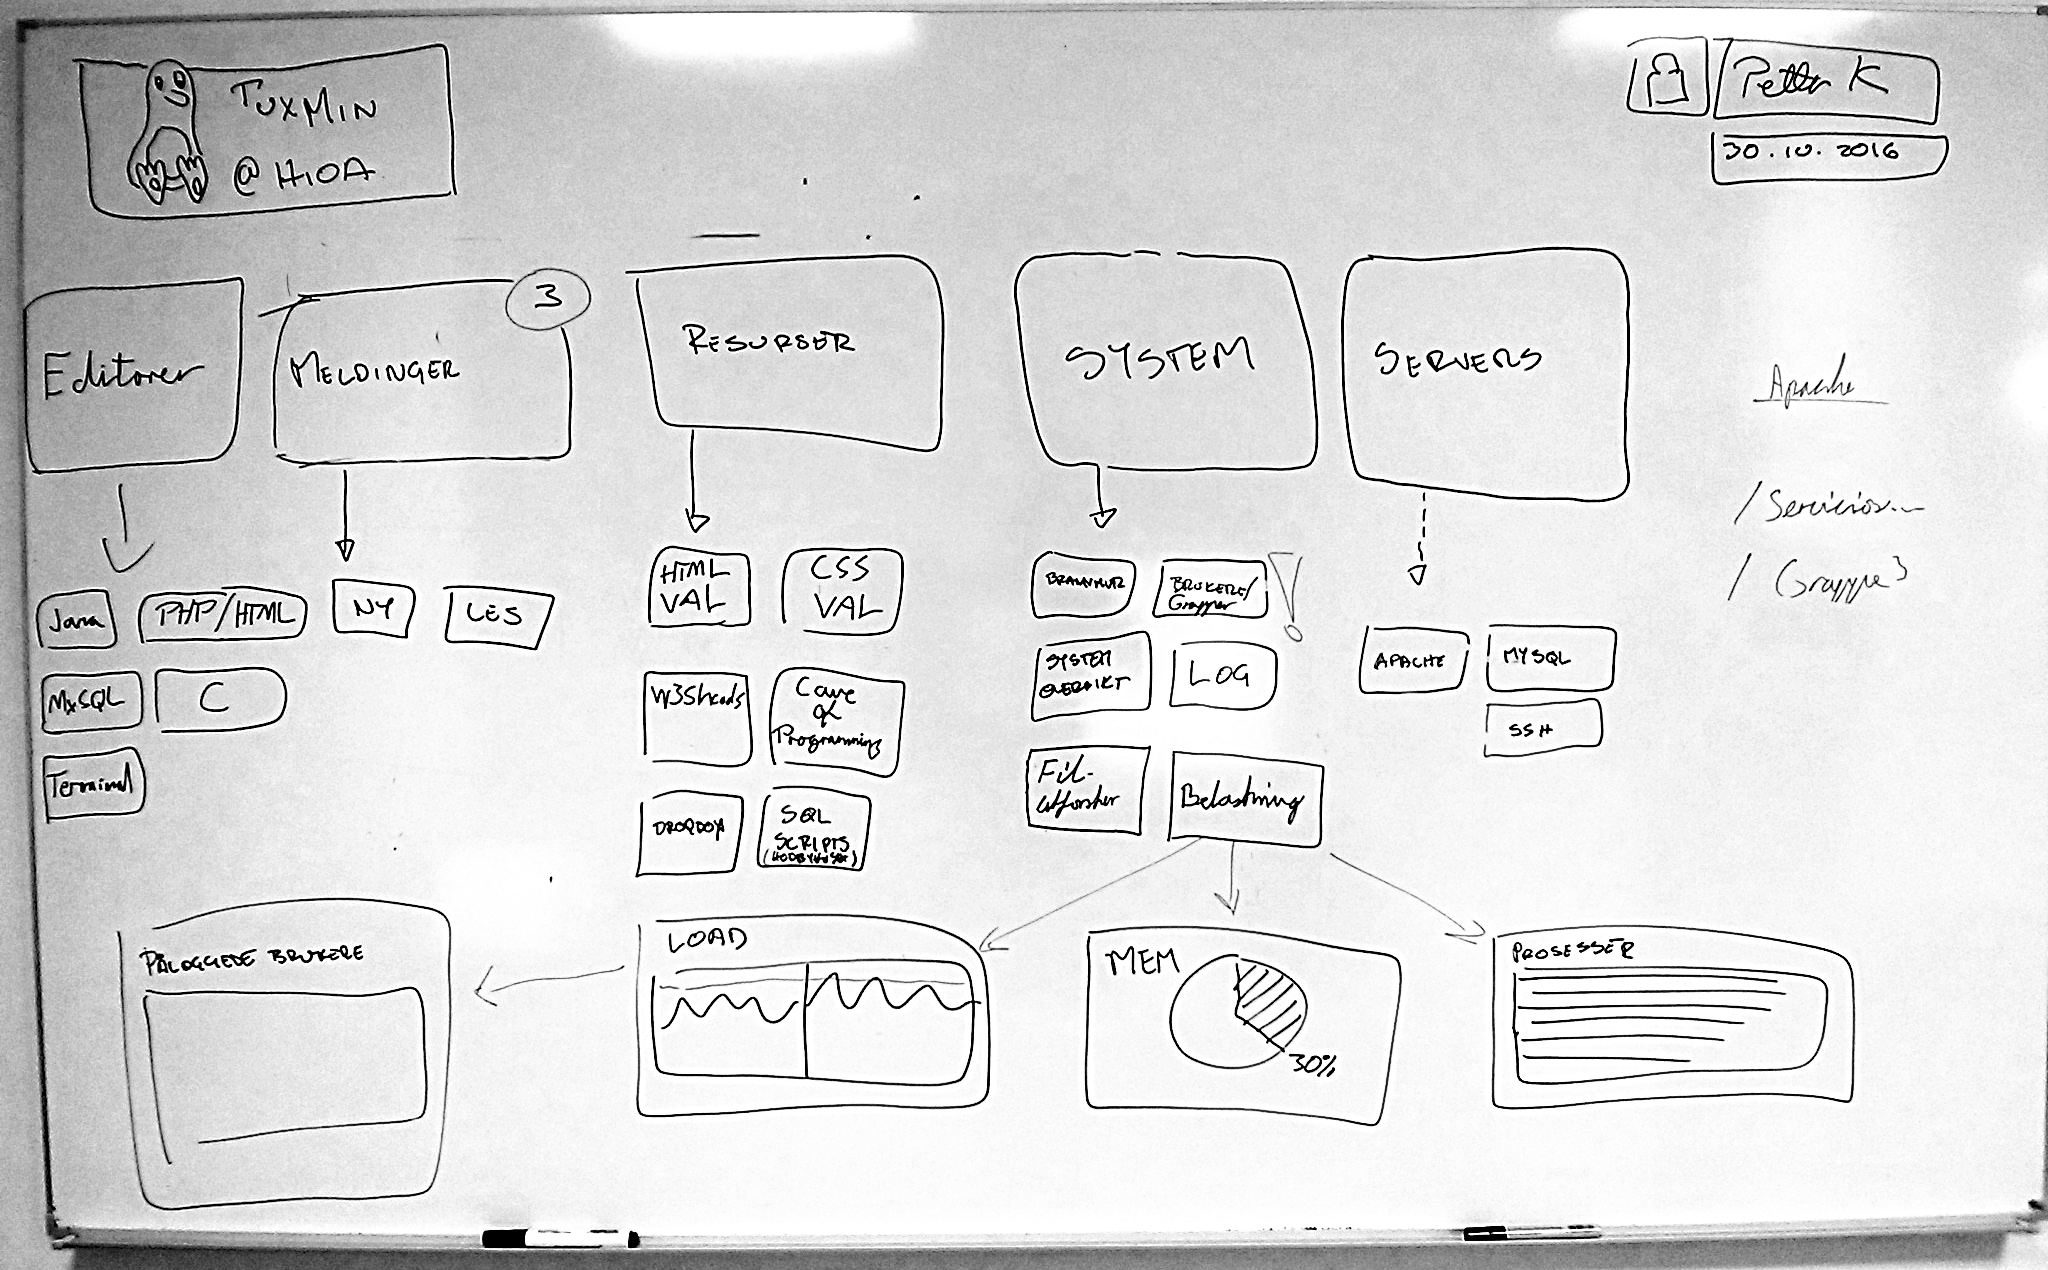
\includegraphics[width=\textwidth,height=\textheight,keepaspectratio]{./img/prosessdokumentasjon/foersteutkast/foerste.jpg}
\caption[Første utkast]{Første utkast over brukergrensesnittet.}
\label{fig:foersteutkast}
\end{figure}

\section{Low-fi prototype} \label{sec:lowfi}
\emph{Avsnittet inneholder et stort antall mockups som representerer forskjellige skjermbilder. Det er flere bilder som er plassert i teksten, og dersom noen av komponentene i bildene oppleves for små er samtlige av bildene presentert i høy oppløsning i appendiks \ref{sec:appendiksLowFi} side \pageref{sec:appendiksLowFi}.}

Det er ganske vanlig at man til en low-fi prototype bruker papp eller papir for å visualisere hvordan man kan bruke en GUI. Vi valgte å benytte oss av \href{http://balsamiq.com/products/mockups/}{balsamiq mockups} som ga oss mulighet til å ikke bare visualisere hvordan brukergrensesnittet skulle se ut men også legge inn enkel funksjonalitet. Blant annet at man fikk mulighet til å klikke seg videre til neste skjermbilde direkte ved å trykke på fra menyer eller knapper i mockupen. Dette ga en ganske grei opplevelse av hvordan det kommer til å føles når man bruker produktet.


Dersom vi tar et rask overblikk over framsiden i figur \ref{fig:lowfi_fremside} ser vi at hver enkelt modul er gruppert etter gestalt prinsipper for proksimitet og elementer.\cite{forelesning:tulpesh}

Prototypen inkluderer eksempel på konfigurasjon av to forskjellige funksjoner.
Det er vanlig at i en prototype fokuserer man på en horisontal eller vertikal implementasjon. Der man i en horisontal implementasjon implementerer få eller ingen funksjoner som går i dybden med istedet forsøker man å vise bredden av muligheter i et system eller grensesnitt. I den vertikale implementasjonen velger man istedet å begrense bredden på hva prototypen kan vise eller gjøre og istedet implementerer en eller flere funksjoner i dybden.\cite{book:utforming}
Vi valgte å avgrense til implementasjon av Apache webserver og oppsett av brukere og grupper. 

\begin{figure}
%bruk \begin{figure}[ht] dersom figuren ikke skal flyte
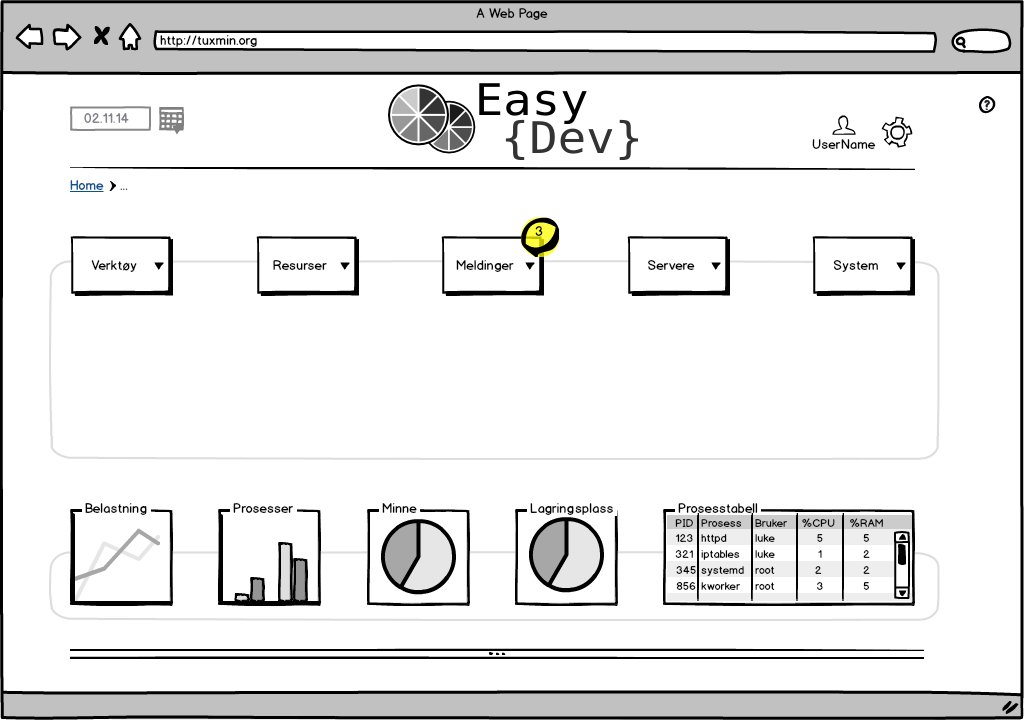
\includegraphics[width=\textwidth,height=\textheight,keepaspectratio]{./img/prosessdokumentasjon/lowfi/fremside.png}
\caption[Low-fi prototype]{Fremside for EasyDev i første low-fi prototype.}
\label{fig:lowfi_fremside}
\end{figure}


I påfølgende avsnitt beskriver vi i detalj funksjonaliteten til to moduler. Det er grunnlegende moduler i systemet og som har vært med siden den opprinnelige idéen ble unnfanget. De to modulene er gode eksempler på hvordan vi har tenkt at produktet skal fungere.

\subsection{Oppsett av apache webserver}
Her går vi nærmere inn på hvordan det er tenkt at en submodul for konfigurasjon og oppsett av serverelement skal brukes. Alle trinn som beskrives er presentert i figur \ref{fig:lowfiapache}.

Vi utgår fra at det er intuitivt å velge modul \texttt{Servere} dersom man ønsker å konfigurere en tjener. Modulen ligger i hovedmenyen med en nedtrekksmeny som viser hvilke servere man har mulighet til å konfigurere, figur \ref{fig:apache1}. 
Apache webserver trenger å vite hvilke mapper som skal deles ut som webområder. Hvis man installerer apache på en Linux manskin kommer den som standard å lese fra mappe \texttt{/var/www} og som har kun root tilgang. Vi vil ikke endre rettigheter for denne mappe ettersom de vi stride mot standarden for rettigheter i systemet og utgjøre en sikkerhetsrisiko.\cite{book:unixprog}
Det vi ønsker å gjøre istedet er å definere om innstillinger i Apache slik at serveren leser fra brukerens sin egen mappe. Dette er normalt en utfordring ettersom det må gjøres i form av to til tre trinn:\footnote{Antall trinn her er ganske avhengig av hvilket Linux system som brukes}

\begin{itemize}
\item Endre konfigurasjon i apache.conf til å lese fra brukerens hjemmemappe. Det må opprettes en spesifikk mappe f.eks. \texttt{/home/bruker/html}. 
I noen tilfelder er det nødvendig å installere plugin \href{http://httpd.apache.org/docs/2.2/mod/mod_userdir.html}{\texttt{mod\_{}userdir}}. Dette vil gjøre det mulig å lese filene vis følgende adresse: \texttt{http://localhost/\~{}bruker/fil.html}

\item Endre rettigheter til den mappen i hjemmemappen som filene skal leses fra. Dette forutsetter at brukeren og Apache webserver er i samme brukergruppe. Oftest må brukeren bli lagt til \texttt{www} eller \texttt{httpd} gruppe på systemet. Det er selvfølgelig mulig å åpne mappen helt, slik at alle grupper i systemet vil ha tilgang til denne, men slik tilnærming senker sikkerheten i stor grad i et flerbrukersystem. Dette er noe som kan være veldig vanskelig for nybegynnere, der man i starten faktisk velger å åpne mappen helt ettersom man ofte ikke greier å teste om rettighetene er satt riktig.

\item Systemer som benytter seg av SELinux (\href{http://en.wikipedia.org/wiki/Security-Enhanced_Linux}{Security Enhanced Linux}) må i tillegg legge til en policy der Apache skal få lov til å lese fra brukermapper. Dette er på grunn at SELinux er et oppsett av rettigheter som i tillegg overstyrer vanlig skriv og leserettigheter i systemet på kernel nivå\footnote{Dette er ikke noe som vi skal beskrive i detalj og nevnes her kun for å illustrere problemstillingen som brukeren kan bli utsatt for.}. 
\end{itemize}

Eksemplene over viser hvor vanskelig det kan være å faktisk sette opp Apache webserver på sin egen maskin.  
Dette er et godt eksempel på hvor EasyDev kommer inn med enkle løsninger. Apache modulen i EasyDev er tiltenkt brukt slik at alle disse konfigurasjonene blir tatt hånd om av systemet, og brukeren har et enkelt grensesnitt å forholde seg til.

Dersom vi ser i figur \ref{fig:apache2} ser vi at i konfigurasjonen kan brukeren velge hvilke mapper som skal inkluderes som et webområde. Altså mapper som webserveren lese fra og vise som websider.
I neste trinn (figur \ref{fig:apache3}) blir brukeren presentert for hvilke av de valgte mappene man ønsker man å benytte for å aktivere <<directory browsing>>. Dette er en funksjon som gjør det mulig å se innholdet i en mappe direkte i nettleseren. Dette er normalt en funksjon som ikke brukes på en <<live>> server men er meget brukbart ved både utvikling og testing. 
Figur \ref{fig:apache4} viser hvilke typer plugins som kan velges som tillegg i Apache installasjonen. Disse kan for eksempel være plugins som PHP eller MySQL eller andre. Hensikten er at man kan samle alle slike tillegg på en plass slik at brukeren kan velge disse på et senere tidspunkt.
Siste eksempel (figur \ref{fig:apache5}) viser mulighet for konfigurasjon av noen av mer avanserte tilleggsmoduler. Disse kan f.eks. være støtte for flere vituelle servere av Apache noe som gir bedre skalerbarhet ved utvikling av flere prosjekter parallelt. 
% med flagg p setter vi hele denne figuren på en egen side
\begin{figure}[p]
        \centering
        \begin{subfigure}[b]{0.48\textwidth}
                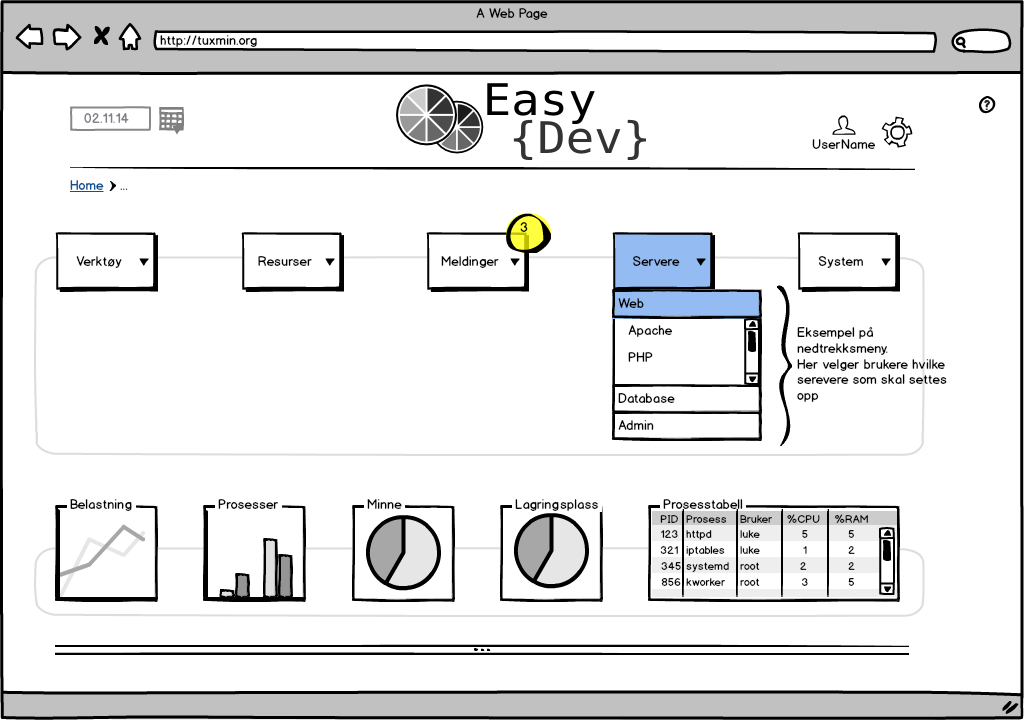
\includegraphics[width=\textwidth]
                {./img/prosessdokumentasjon/lowfi/apache1.png}
                \caption{Fremside -> Sett opp webserver}
                \label{fig:apache1}
        \end{subfigure}%
        ~ %add desired spacing between images, e. g. ~, \quad, \qquad, \hfill etc.
          %(or a blank line to force the subfigure onto a new line)
        \begin{subfigure}[b]{0.48\textwidth}
                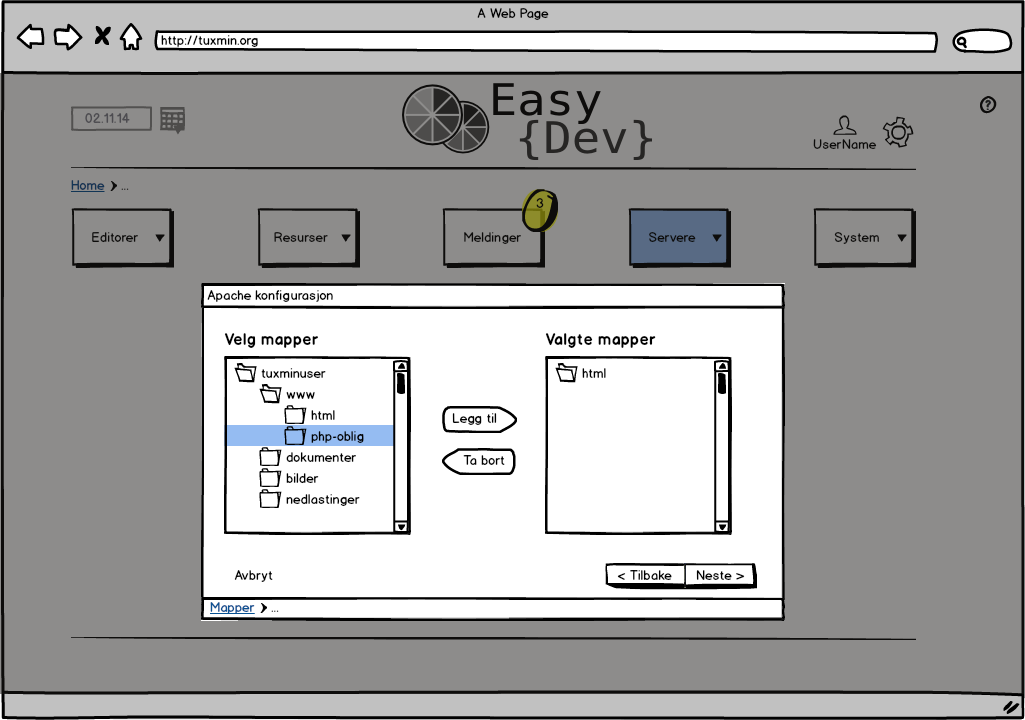
\includegraphics[width=\textwidth]
                {./img/prosessdokumentasjon/lowfi/apache2.png}
                \caption{Valg av mapper}
                \label{fig:apache2}
        \end{subfigure}
       
        \vspace{0.6cm}
        \begin{subfigure}[b]{0.48\textwidth}
                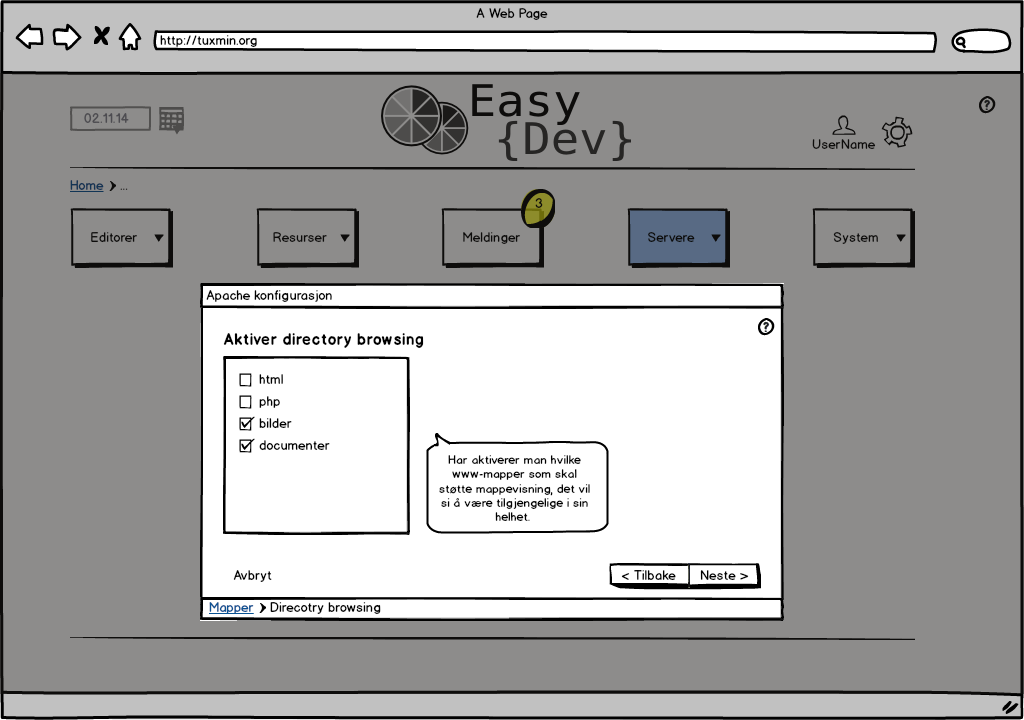
\includegraphics[width=\textwidth]
                {./img/prosessdokumentasjon/lowfi/apache3.png}
                \caption{Aktivere visning av innhold i mapper}
                \label{fig:apache3}
        \end{subfigure}
        \hspace{0.05cm}
        \begin{subfigure}[b]{0.48\textwidth}
                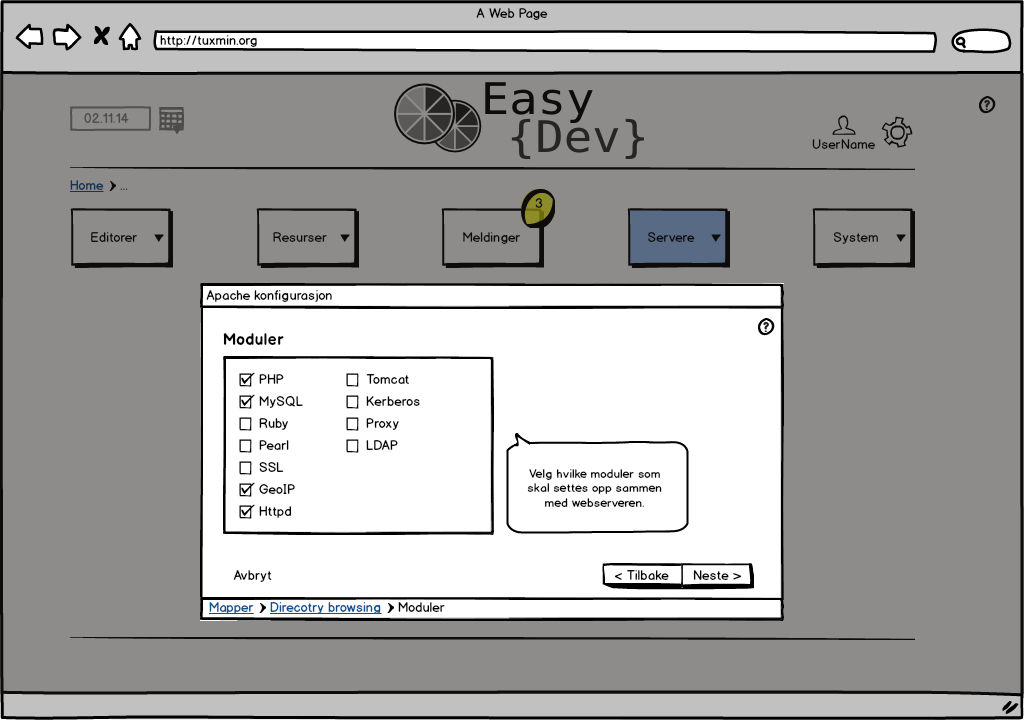
\includegraphics[width=\textwidth]
                {./img/prosessdokumentasjon/lowfi/apache4.png}
                \caption{Valg av moduler}
                \label{fig:apache4}
        \end{subfigure}
        
        \vspace{0.6cm}
        \begin{subfigure}[b]{0.48\textwidth}
                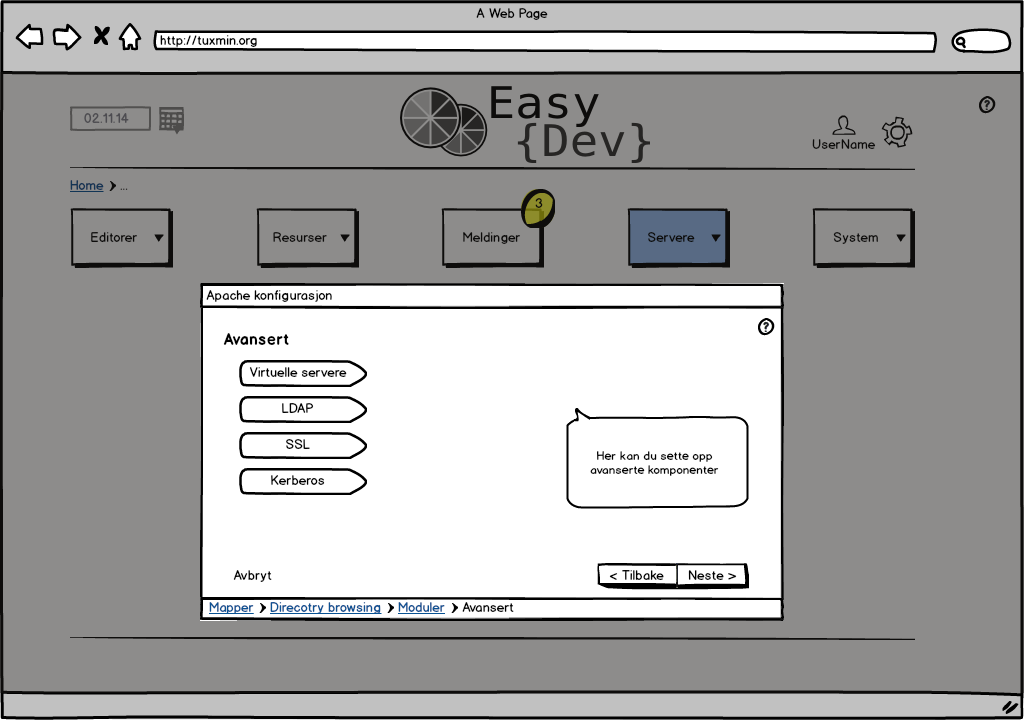
\includegraphics[width=\textwidth]
                {./img/prosessdokumentasjon/lowfi/apache5.png}
                \caption{Avanserte Apache moduler}
                \label{fig:apache5}
        \end{subfigure}
        \vspace{0.1cm}
        \caption[Konfigurasjon av Apache webserver]{Eksempel på konfigurasjon av Apache webserver.}\label{fig:lowfiapache}
\end{figure}


\subsection{Oppsett av brukere og grupper}
I følgende modul har man mulighet til å sette både brukergrupper, brukere og rettigheter en en enkelt bruker eller hele grupper av brukere. Modulen er tenkt å brukes i forbindelse med gruppearbeid slik at flere brukere kan dele på samme resurser. De eksempler som beskrives her kan betraktes i figur \ref{fig:lowfibrukere}. 
% med flagg p setter vi hele denne figuren på en egen side
\begin{figure}[h]
        \centering
        \begin{subfigure}[b]{0.48\textwidth}
                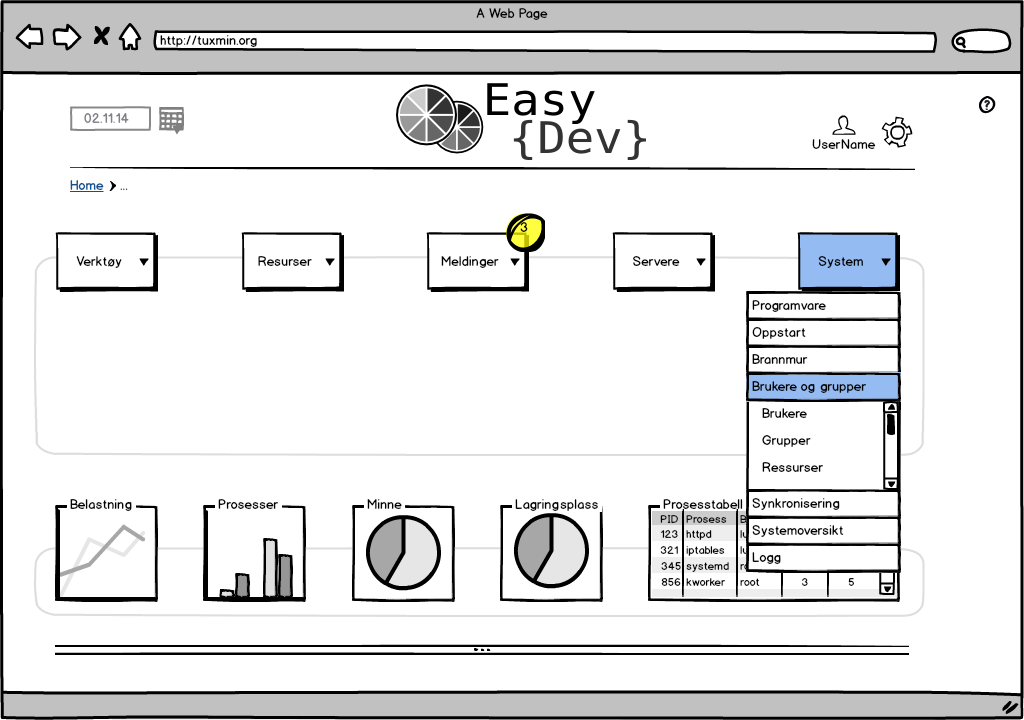
\includegraphics[width=\textwidth]
                {./img/prosessdokumentasjon/lowfi/b1.png}
                \caption{Fremside -> Velg brukeroppsett}
                \label{fig:brukere1}
        \end{subfigure}%
        ~ %add desired spacing between images, e. g. ~, \quad, \qquad, \hfill etc.
          %(or a blank line to force the subfigure onto a new line)
        \begin{subfigure}[b]{0.48\textwidth}
                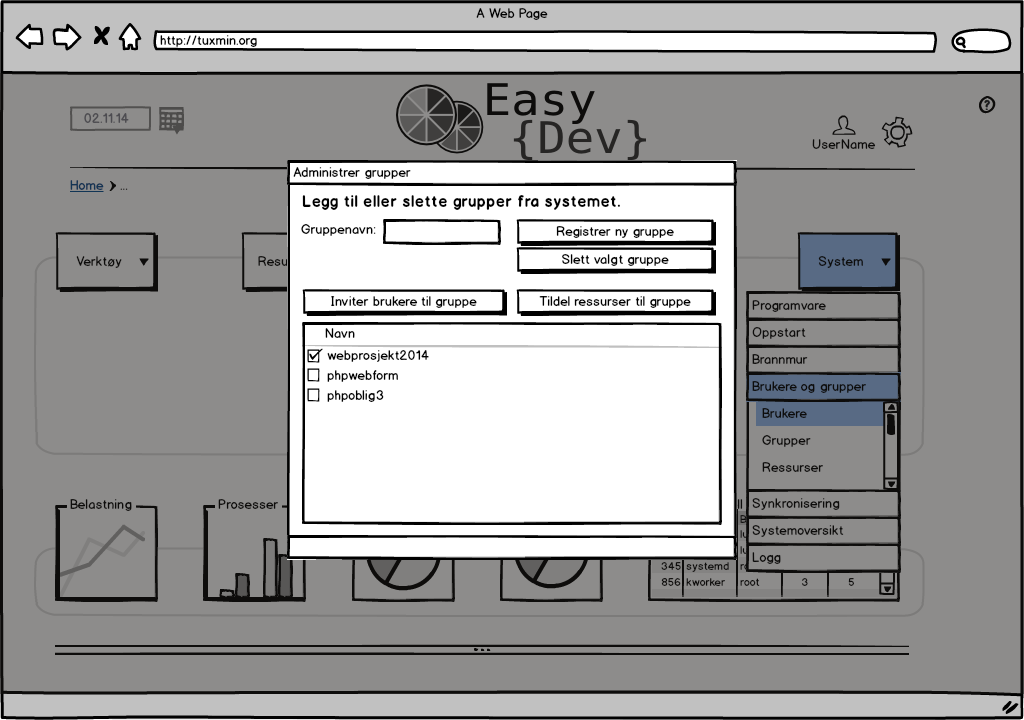
\includegraphics[width=\textwidth]
                {./img/prosessdokumentasjon/lowfi/b2.png}
                \caption{Grupper}
                \label{fig:brukere2}
        \end{subfigure}
       
        \vspace{0.4cm}
        \begin{subfigure}[b]{0.48\textwidth}
                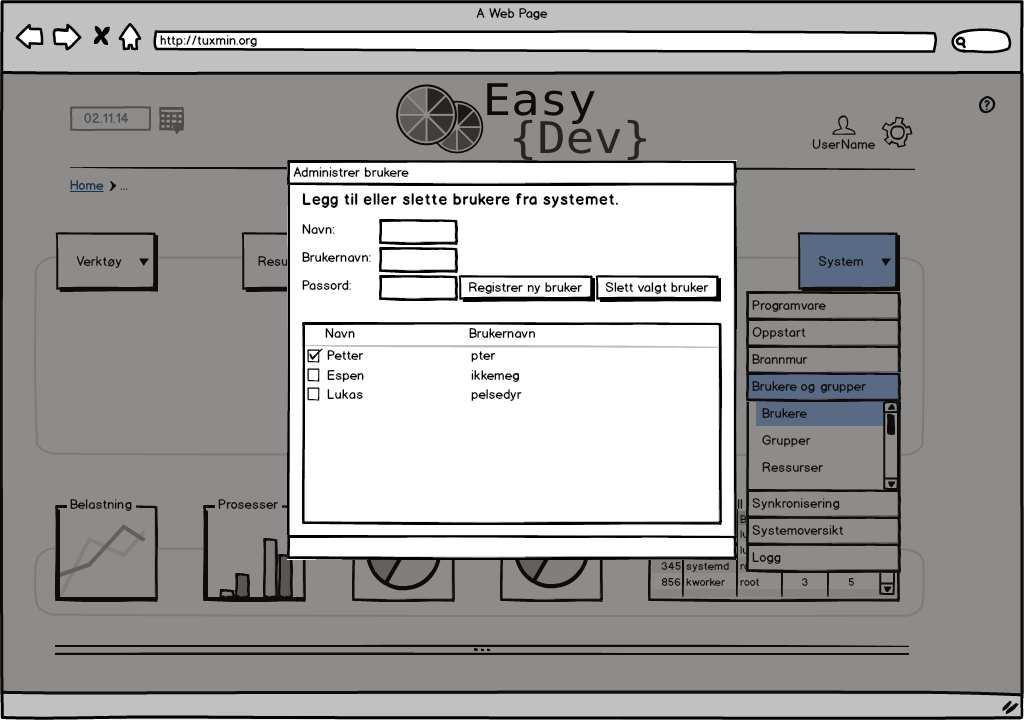
\includegraphics[width=\textwidth]
                {./img/prosessdokumentasjon/lowfi/b3.png}
                \caption{Brukere}
                \label{fig:brukere3}
        \end{subfigure}
        \hspace{0.02cm}
        \begin{subfigure}[b]{0.48\textwidth}
                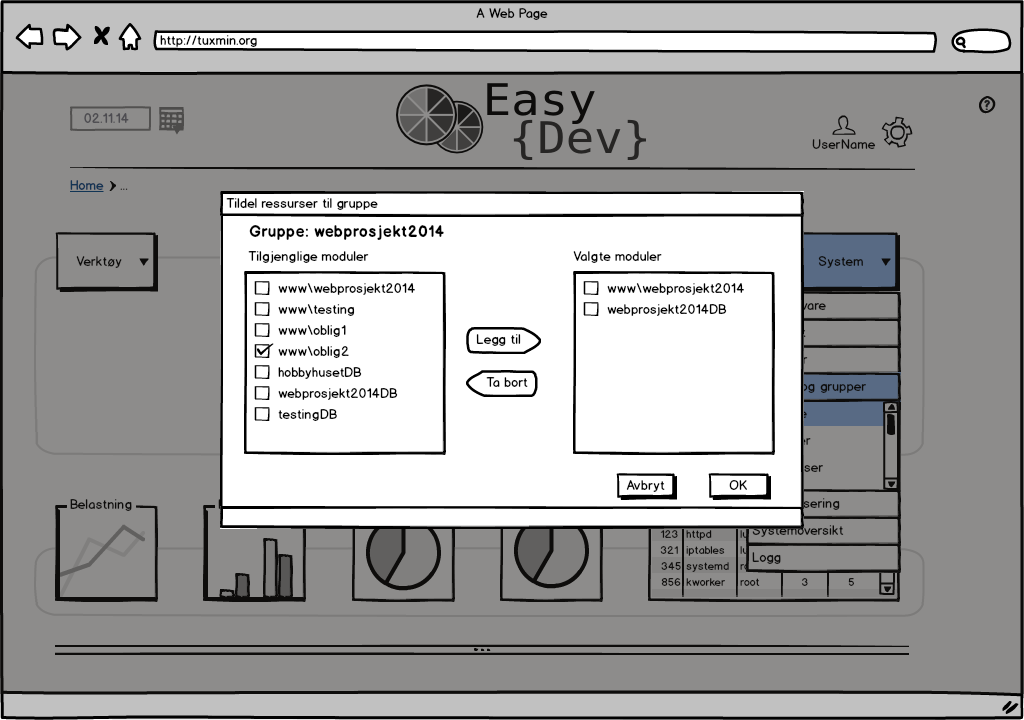
\includegraphics[width=\textwidth]
                {./img/prosessdokumentasjon/lowfi/b4.png}
                \caption{Moduler og resurser for gruppe}
                \label{fig:brukere4}
        \end{subfigure}
        \vspace{0.1cm}
        \caption[Konfigurasjon av brukere og grupper]{Eksempel på konfigurasjon av brukere og grupper.}\label{fig:lowfibrukere}
\end{figure}
Vi begynner på samme måte som i forrige eksempel og starter på fremsiden (figur \ref{fig:brukere1}). I stedet for å velge modulen <<Servere>> går vi til modul <<System>> som innholder flere undermoduler som kan brukes til oppsett og konfigurasjon av selve den virtuelle maskinen og brukergrensesnittet. 
Vi kan deretter (figur \ref{fig:brukere2}) sette opp en ny gruppe, slette gruppe eller gå videre med å legge til brukere til en gruppe. Vi også se hvilke ressurser som allerede er tildelt en gruppe og eventuelt kan vi fjerne disse rettighetene ved å ta haken et eller flere av alternativene.\\
Dersom vi ønsker å legge til nye brukere i systemet vårt kan vi gjøre det i neste skjermbilde (figur \ref{fig:brukere3}) og på en enkel måte gå videre og legge til eller slette brukere.
Hvis vi ønsker kan vi gå videre til neste skjermbilde og legge til nye ressurser som skal være tilgjengelige for en spesifikk gruppe. Dette kan f.eks. dreie seg om en database, et webområde eller lignende, der alle som er medlem i en gruppe har tilgang.

\section{Hi-fi prototype}
\emph{Følgende avsnitt inneholder ikke figurer av all funksjonalitet i hi-fi prototypen. Det er et flertall skjermbilder som må vises i full bredde. Derfor er samtlige hi-fi mockup flyttet til appendiks \ref{sec:appendiksHiFi} side \pageref{sec:appendiksHiFi}.}

Hi-fi prototypen er en videreutvikling av tidligere prototype som er gjort med hjelp av samme verktøy som skal brukes til ferdig produkt. Ved utvikling av hi-fi prototype ble det brukt  html, css, javascript og php for å sy sammen funksjonalitet og få den til å fungere som en nettside. I figur \ref{fig:hifi_fremside} ser man hvordan fremsiden blir presentert. Dette kan gjerne sammenliknes med den tidligere mockupen figur \ref{fig:lowfi_fremside} side \pageref{fig:lowfi_fremside}. Det er ikke bestemt hva som skal vises på fremsiden enda, men mest sannsynlig blir det meldinger fra lærer og de man jobber i gruppe med.
\begin{figure}[ht]
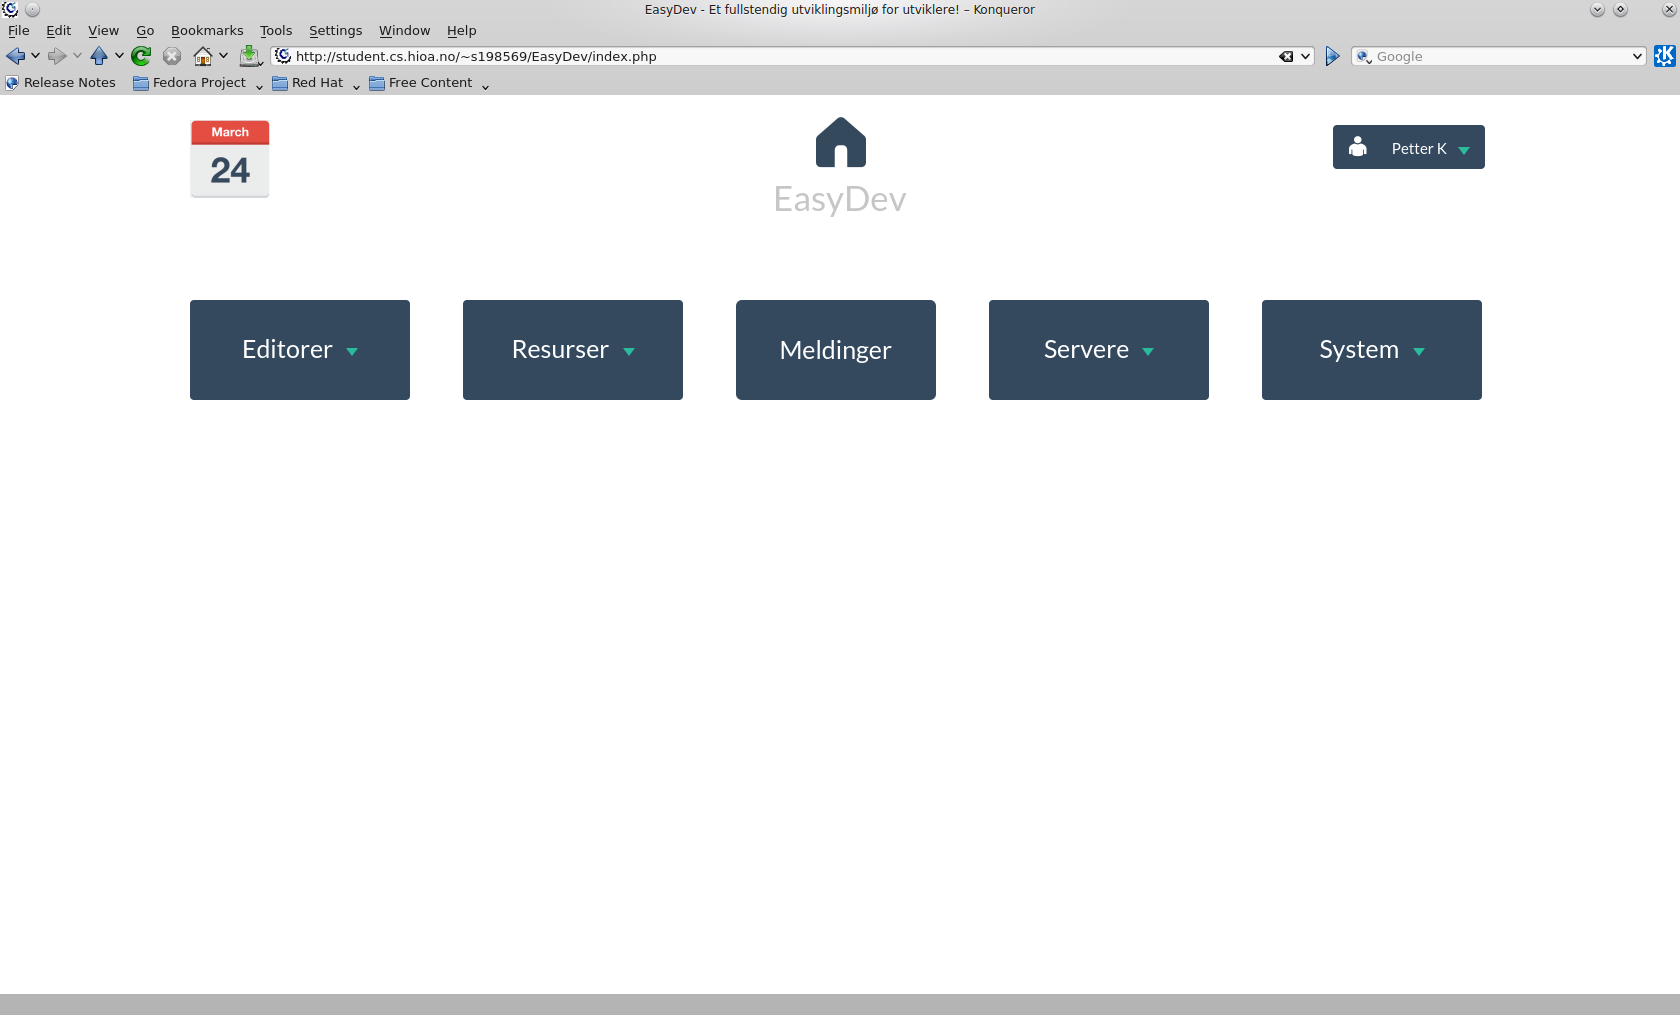
\includegraphics[width=\textwidth,height=\textheight,keepaspectratio]{./img/prosessdokumentasjon/hifi/fremside.png}
\caption[Hi-fi prototype]{Fremside for EasyDev som hi-fi prototype.}
\label{fig:hifi_fremside}
\end{figure}

Det er en litt annerledes tilnærming til hvordan dialogvinduene til brukeren blir presentert i denne prototypen. Se figur \ref{fig:hifi_brukerdialog}. Dialogen blir presentert lengre ned i forhold til den hovedmenyen som medfører at store deler av det tomme området på fremsiden blir i stedet brukt for visning av dialoger. 

\begin{figure}[ht]
\centering
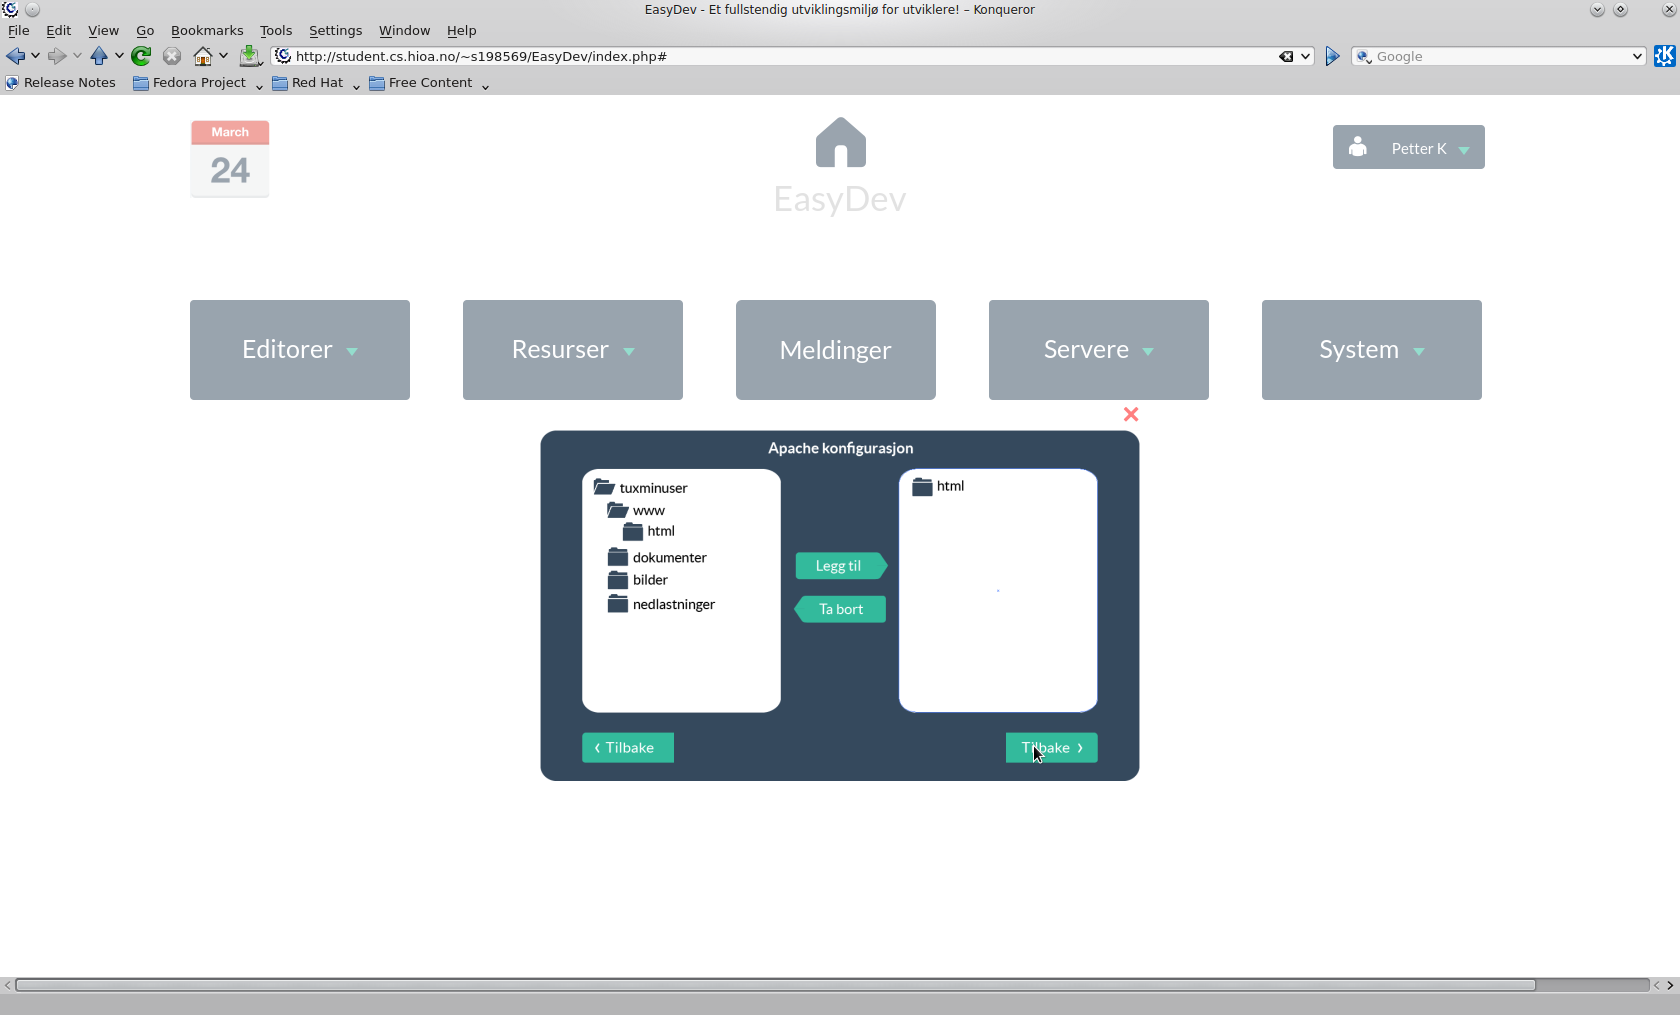
\includegraphics[width=0.8\textwidth,keepaspectratio,trim = {12cm 6cm 12cm 8cm}, clip]{./img/prosessdokumentasjon/hifi/a2.png}
\caption[Hi-fi brukerdialog]{Eksempel over fremstilling av brukerdialog. Utklippet viser eksempel på ny design hvor dialogen er plassert i forhold til menyen.}
\label{fig:hifi_brukerdialog}
\end{figure}

\section{Kriterier og avgjørelser}
Følgende avsnitt beskriver hvilke og hvorfor vi har tatt de valg som vi har gjort under reisen. Vi skal fokusere på valg kriterier og valg fra et MMI perspektiv men det er også viktig å opplyse av andre kriterier som mer teknisk karakter.

\subsection{Virtuell maskin}
System skal kjøre i en vituell maskin ettersom det er enkelt å både opprette slette eller gjenopprette slik løsning. Da en ny bruker skal starte en maskin trenger denne kun å bli kopiert fra et image og satt opp med riktig brukernavn og passord. Dersom brukeren ødelegger noe i maskinen er det mulig å eksportere konfigurasjonsfiler for valgte moduler og opprette en ny maskin sammen med eksisterende konfigurasjonfiler, til f.eks. Apache.

\subsection{Webbasert}
Ettersom grensesnittet er webbasert blir det tilgjengelig fra hvilken datamaskin som helst uavhengig operativsystem eller nettleser. Systemet vil få en god skalering da det blir enkelt å sette inn eller fjerne moduler. Det vil også være relativ liten terskel for studenter å utvikle egne moduler dersom man synes at noen moduler mangler i systemet. 

\subsection{Bruk av visuelle elementer}
Som tidligere beskrevet i avsnitt \ref{sec:utkast} og \ref{sec:lowfi} har vi valgt å benytte oss av gestalt prinsipper ved plassering av alle visuelle komponenter. Hensikten er at når brukeren for første gang logger på systemet skal man kunne bruke det helt intuitivt og uten å behøve tenkte på hvordan det er implementert.

Et godt eksempel på dette er plassering av alle knapper på fremsiden. Disse har vi valgt å legge horisontalt med samme avstand fra hverandre. Slik plassering danner tilhørighet, man vet at disse henger sammen (\textit{proximity, element connectedness, similarity}). I tillegg forsterkes dette gjennom at vi bruker samme farger på alle de komponentene.\cite{forelesning:tulpesh}. Vi vil gå videre med disse prinsippene ved eventuell videreutvikling av systemet slik at man kunne fargekodet de forskjellige områdene slik at hver område er lett identifiserbart grunnet disse fargekodene. 
Samme prinsipper gjelder også for de undermenyer som åpnes dersom man klikker på noen av de komponentene. Man blir presentert med en liste av muligheter gruppert etter tilhørighet til sin funksjon. 

Toppmenyen er symmetrisk distribuert for å danne en følelse balanse og sentral plassering i layouten. Vi har plassert EasyDev logo i midten og på begge sider av den, komponenter som er kalender og klokke til venstre samt brukerikonet og hurtigvalg til innstillinger til høyre for logoen. 

\subsection{Bruk av farger}
Vi har konsekvent valgt å avgrense oss til grunnpaletten i \textit{FlauUI} grensesnittet. Alle farger som vi kan bruke i løsningen presenteres i form av en matrise i figur \ref{fig:farger}. Dette er $4\times 5$ matrise som kanskje bare har tilgang til tjue farger men gir oss ganske store muligheter. 
\begin{figure}[h]
\begin{tabularx}{\textwidth}{*6{>{\centering\arraybackslash}X}@{}}

\cellcolor{Turquoise} \emph{Turquoise} & \cellcolor{Emerald} \textit{Emerald} & \cellcolor{PeterRiver} \emph{Peter River} & \cellcolor{Amethyst} \emph{Amethyst} & \cellcolor{WetAsphalt} \emph{Wet Asphalt} \\[5ex] 

\cellcolor{GreenSea} \emph{Green Sea} & \cellcolor{Nephritis} \textit{Nephritis} & \cellcolor{BelizeHole} \emph{Belize Hole} & \cellcolor{Wisteria} \emph{Wisteria} & \cellcolor{MidnightBlue} \emph{Midnight Blue} \\[5ex] 

\cellcolor{SunFlower} \emph{Sun Flower} & \cellcolor{Carrot} \textit{Carrot} & \cellcolor{Alizarin} \emph{Alizarin} & \cellcolor{Clouds} \emph{Clouds} & \cellcolor{Concrete} \emph{Concrete} \\[5ex] 
 
\cellcolor{Orange} \emph{Orange} & \cellcolor{Pumpkin} \textit{Pumpkin} & \cellcolor{Pomegranate} \emph{Pomegranate} & \cellcolor{Silver} \emph{Silver} & \cellcolor{Asbestos} \emph{Asbestos} \\[5ex] 

\end{tabularx} 
\caption[Fargekombinasjoner]{Fargekombinasjoner som brukes i hi-fi prototypen}
\label{fig:farger}
\end{figure}
Dersom vi ser på de to øverste og de to nederste radene ser vi at disse bare er forskjellige nyanser av samme farge. Disse har vi valgt å bruke som utheving eller for å danne lav kontrast mellom feks. tabellrader. 
Dersom vi trenger mer kontrast for å varsle brukeren om noe kan vi ta i bruk to \textbf{analoge} farger. Disse er plassert over hverandre i rader 1-3 eller 2-4, f.eks. \emph{Turqoise} og \emph{Sun Flower} eller \emph{Belize Hole} og \emph{Pomegranade}.
Disse gir myke overganger og kan oftest benyttes sammen og gi en myk og fin overgang f.eks. mellom bakgrunnen i et grensesnitt og et element som f.eks. en knapp.
Til sist er det også mulig å benytte seg av to \textbf{komplementærfarger}.
Disse har vi plassert på skrå fra hverandre som \emph{Peter River} og \emph{Orange} eller \emph{Amethyst} og \emph{Sun Flower}. Disse fargene kombinert brukes til å tydelig markere overgangen mellom et objekt og et annet.

Generelt har vi selvsagt ikke benyttet oss av alle disse farger i hi-fi prototypen da mange av dem blir reservert til spesielle tilfeller. Kun mer monotone av farger i figur \ref{fig:farger} blir brukt til komponenter og bakgrunner som ofte forekommer i komponentene.

\subsection{Open Source}
Vi har valgt å basere vår løsning kun på produkter som er tilgjengelige via open source eller som fri kode. Dette er ganske viktig da prosjektet som kunne videreutvikles og ikke skal være avhengig av proprietær teknologi. Videre skal vår kildekode gjøres tilgjengelig slik at det kan gjøres endringer og forbedringer på eksisterende moduler eller lages nye (se avsnitt \ref{sec:hjelpogverkt} for linker). 
